%!TEX root = ../Thesis.tex
\chapter{On Local Posterior Structure in Deep Ensembles}
\label{chap:AISTATS}
In this chapter, I present our paper "On Local Posterior Structure in Deep Ensembles" which is currently under review at AISTATS 2025. This work started for primarily from a mixture of two reasons. Firstly, Jonas and I had for a while time been discussing about the difficulty of getting some approximate inference methods to work in practice and therefore wanted to experiment with some of these methods on datasets that are not so commonly seen in the literature. Secondly, we were curious to see if anything could be said about including local posterior structure in deep ensembles (DEs), discussed in Section \ref{sec:DEs}. Moreover, we were interested to see if the performance of such models could be improved by methodological proposals such as alternatives to Monte-Carlo sampling in the posterior predictive or complex stacking methods, for example pruning of networks in the ensemble that were functionally similar. Surprisingly, we found that normal DEs outperformed ensembles of BNNs (DE-BNNs) when the ensembles sizes became large enough, leading to this paper which is largely empirical and shines a new light on DE-BNNs in contrast to previous works \citep{2021_MOLA, 2020_MultiSWAG}.\\

\noindent In this work, we apply approximate inference methods, specifically Last Layer Laplace (see Section \ref{sec:LAPLACE}) and SWAG (see Section \ref{sec:SWAG}), to Bayesian neural networks on several datasets, including some that we have not previously seen in the literature and systematically investigate if DE-BNNs provide additional uncertainty quantification benefits over DEs. For single models we, similar to previous works, confirm that BNNs improve on the uncertainty quantification and calibration of MAP estimated neural networks without impacting accuracy. We then show that when we compose DE-BNNs they for small ensemble sizes outperform regular DEs both on in-distribution and out-of-distribution metrics, but that when the ensembles grow large enough, DEs outperform DE-BNNs on in-distribution metrics. We then show that even though DE-BNNs perform better on out-of-distribution metrics for large ensemble sizes, this comes at a cost of in-distribution performance. We investigate why this counter-intuitive behaviour occurs and discuss potential future investigations that could try to remedy this problem of DE-BNNs.

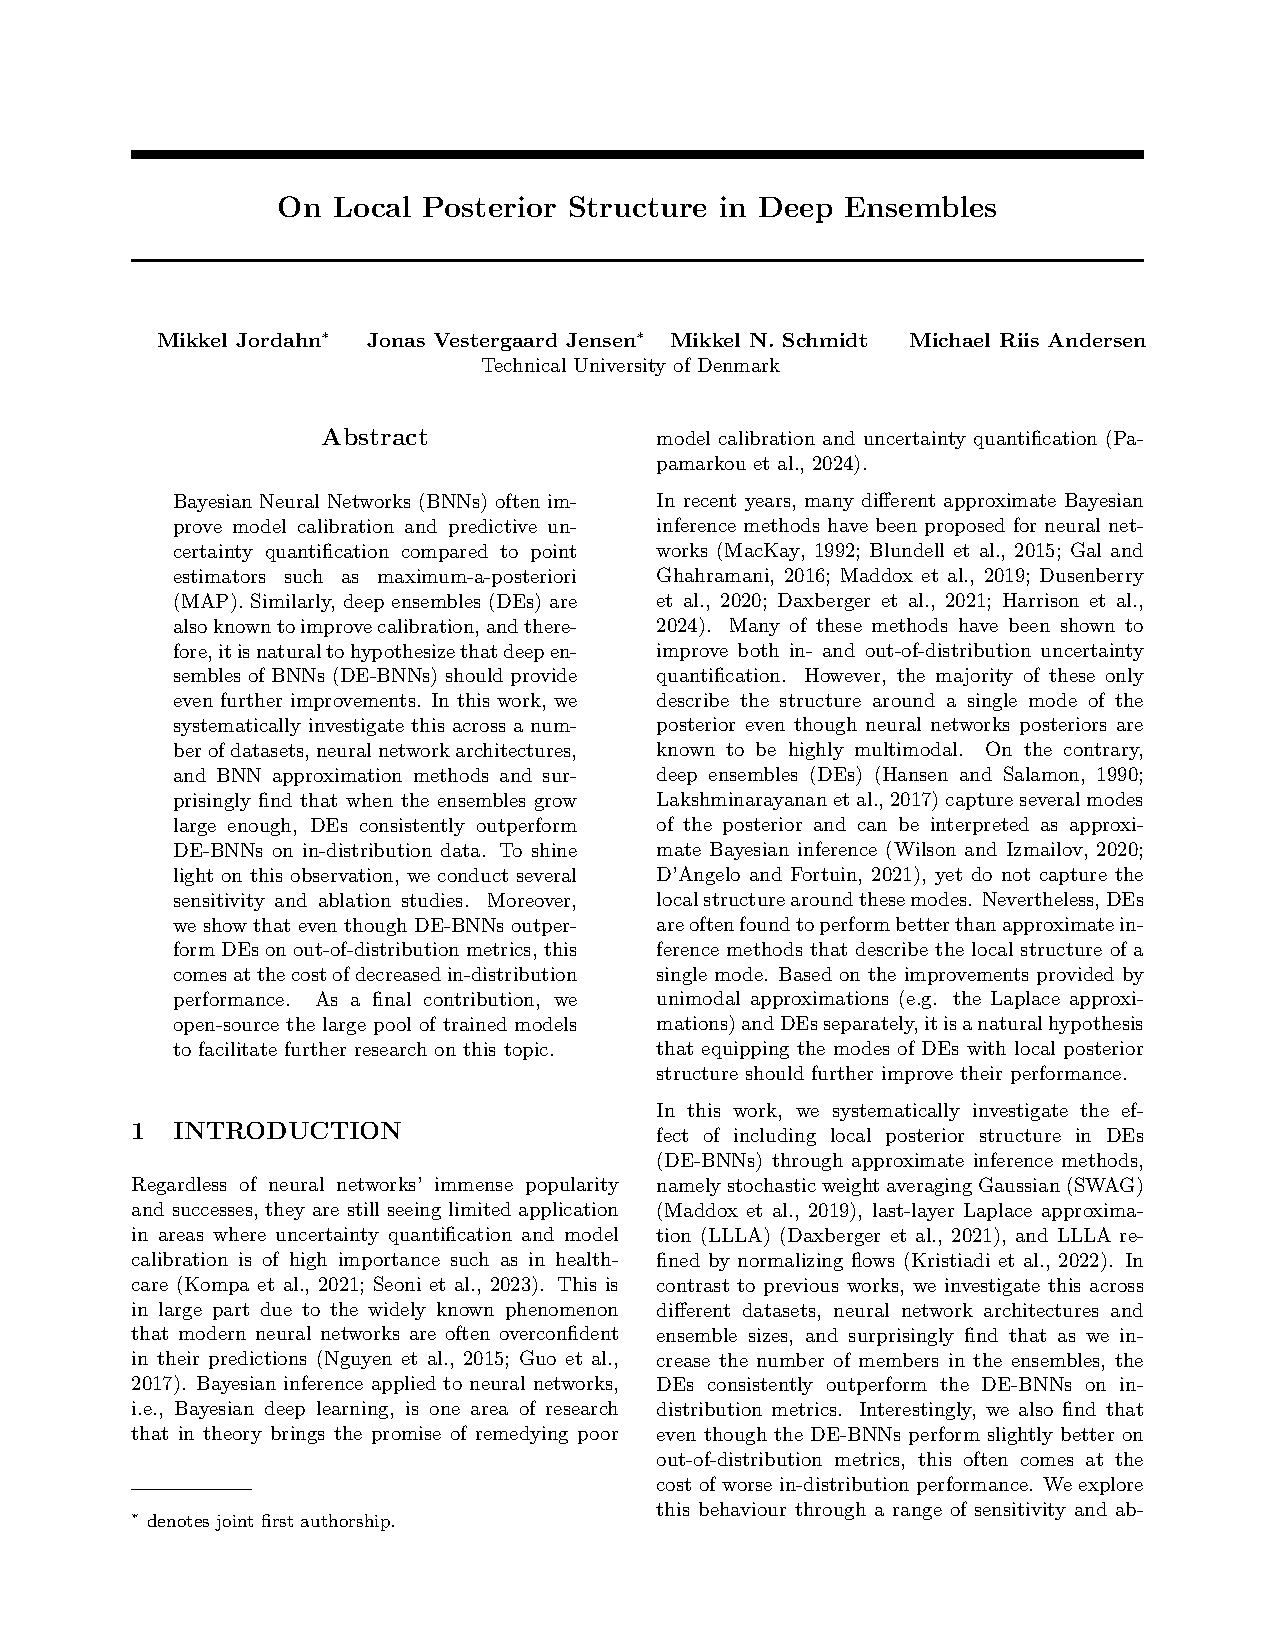
\includepdf[pages=-, offset=0mm 0mm, delta=0mm 0mm, scale=1.0, pagecommand={\thispagestyle{mystuff}{}{}{}}]{chapters/paperB_DE/AISTATS2025.pdf}